\documentclass[11pt]{scrartcl}
\usepackage{fullpage}

\usepackage{listings} % Coding Syntax coloring
\usepackage{color}
\usepackage{textcomp}
\definecolor{listinggray}{gray}{0.9}
\definecolor{lbcolor}{rgb}{0.9,0.9,0.9}

\usepackage{amsmath}
\usepackage{textcomp}

\lstset{
     backgroundcolor=\color{lbcolor},
     tabsize=4,
     rulecolor=,
     language=matlab,
        basicstyle=\scriptsize,
        upquote=true,
        aboveskip={1.5\baselineskip},
        columns=fixed,
        showstringspaces=false,
        extendedchars=true,
        breaklines=true,
        prebreak = \raisebox{0ex}[0ex][0ex]{\ensuremath{\hookleftarrow}},
        frame=single,
        showtabs=false,
        showspaces=false,
        showstringspaces=false,
        identifierstyle=\ttfamily,
        keywordstyle=\color[rgb]{0,0,1},
        commentstyle=\color[rgb]{0.133,0.545,0.133},
        stringstyle=\color[rgb]{0.627,0.126,0.941},
}
\usepackage{fancyhdr,graphicx,lastpage}% http://ctan.org/pkg/{fancyhdr,graphicx,lastpage}
\fancypagestyle{plain}{
  \fancyhf{}% Clear header/footer
  \fancyhead[R]{
\includegraphics[scale=0.5]{logo.png}}% Right header
  \fancyhead[L]{\textbf{School of Electronic and Electrical Engineering}}
  %\fancyfoot[L]{Name Firstname - v1.0 \\  Date}% Left footer
  \fancyfoot[R]{\thepage\  / \pageref{LastPage}}% Right footer
}
\pagestyle{plain}% Set page style to plain.


\begin{document}
\title{ELEC2856 Assignment 4}
\subtitle{ Audio Signal Processing}
\author{Yingjie Luan}
\maketitle

\tableofcontents


\section{Frequency responses of woofer and tweeter }
\subsection{Experiment setup}

In testing the response of the woofer and the tweeter, we set the height of the speaker and microphone both at 0.62m. And the location of the speaker is approximately at the central line of the room. The room itself is an audio experiment room with soft material all over the room. But we also spotted the imperfection of the room, which are:
\begin{enumerate}
  \item The curtain is not well closed and the glass is capable of reflecting the sound.
  \item There is some highly reflectively plastic wire enclosure wrapped around the room.   
\end{enumerate}

We tested the speaker at two distance(the distance between the speaker and the microphone), the close one is at 1.79m(the speaker is approximately at the center of the room) and the further one is at approximately at 3m(the speaker is at the far back of the room).

For experiment setup, we use the PC to generate the control signal, and clio to translate that signal into audio signal, we then use an amplifier to amplifier that signal to feed in the speaker, and the sound is feed back to the microphone and finally to the PC by clio.

\subsection{Experiment condition}

Clio are used for doing the experiment, the testing method is to generate a range of variable amplitude sinusoidal sound. The frequency range is approximately equals to the human era's range, which is from around 10hz to 22khz. \\

We tested devices as below:
\begin{enumerate}
  \item Twitter: Capable of generating high frequency sound.
  \item Woofer: Capable of generating low frequency sound.
\end{enumerate}

We tested condition as below:
\begin{enumerate}
  \item Bare: Speaker without enclosure.
  \item Baffle: Speaker with a back board as enclosure.
  \item Cabinet: Speaker with a wooden case as enclosure.
\end{enumerate}

We tested in the distance below:
\begin{enumerate}
  \item Close: The distance between speaker and the microphone is at around 1.7m.
  \item Far: The distance between speaker and the microphone is at around 3m.
\end{enumerate}
\subsection{Results}
We get 2*2*3=12 results. Which are below:


\section{Design of the filter}

We implemented two active filters, for both filters, they are composed of 3 individual first order filter. 
\paragraph{low pass filter}
For low pass filter, the transform function is:
$$H(j\omega) = \frac{R/r}{1+j\omega/\omega_H}$$
and:
$$\omega_H=1/(RC)$$
$\omega_H$ is the cutoff frequency at 3db. We set R=r.
\begin{center}
\begin{minipage}[t]{\linewidth}
%\label{fig:main}

{
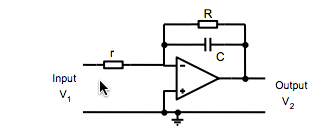
\includegraphics[scale = 1]{low.png}
\captionof{figure}{This is the diagram of the low pass filter.}
}
\end{minipage}
\medskip
\end{center}
\paragraph{high pass filter}
For the high pass filter, the transform function is:
$$H(j\omega) = \frac{-j\omega CR}{1+\omega/\omega_L}$$
and:
$$\omega_L=1/(rC)$$
$\omega_L$ is the cutoff frequency at 3db. We set R=r.

\begin{center}
\begin{minipage}[t]{\linewidth}
%\label{fig:main}

{
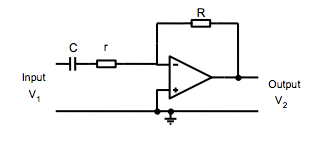
\includegraphics[scale = 1]{high.png}
\captionof{figure}{This is the diagram of the high pass filter.}
}
\end{minipage}
\medskip
\end{center}
\subsection{Requirements for the filter}
We want to design two filters, and the description is below:
\begin{enumerate}
  \item Low pass filter: its crossover frequency is at 2.3khz, it is a 3 order system to guarantee a shaper response than first order system.
  \item High pass filter: its crossover frequency is at 2.3khz, it is a 3 order system to guarantee a shaper response than first order system.
\end{enumerate}

\subsection{The implementation filter}

For implementation, we just feed one first order filter's output to another first order filter's input, and thus we get a 3 order high pass filter and a 3 order low pass filter.

Below is the snapshot:
\begin{center}
\begin{minipage}[t]{\linewidth}
%\label{fig:main}

{
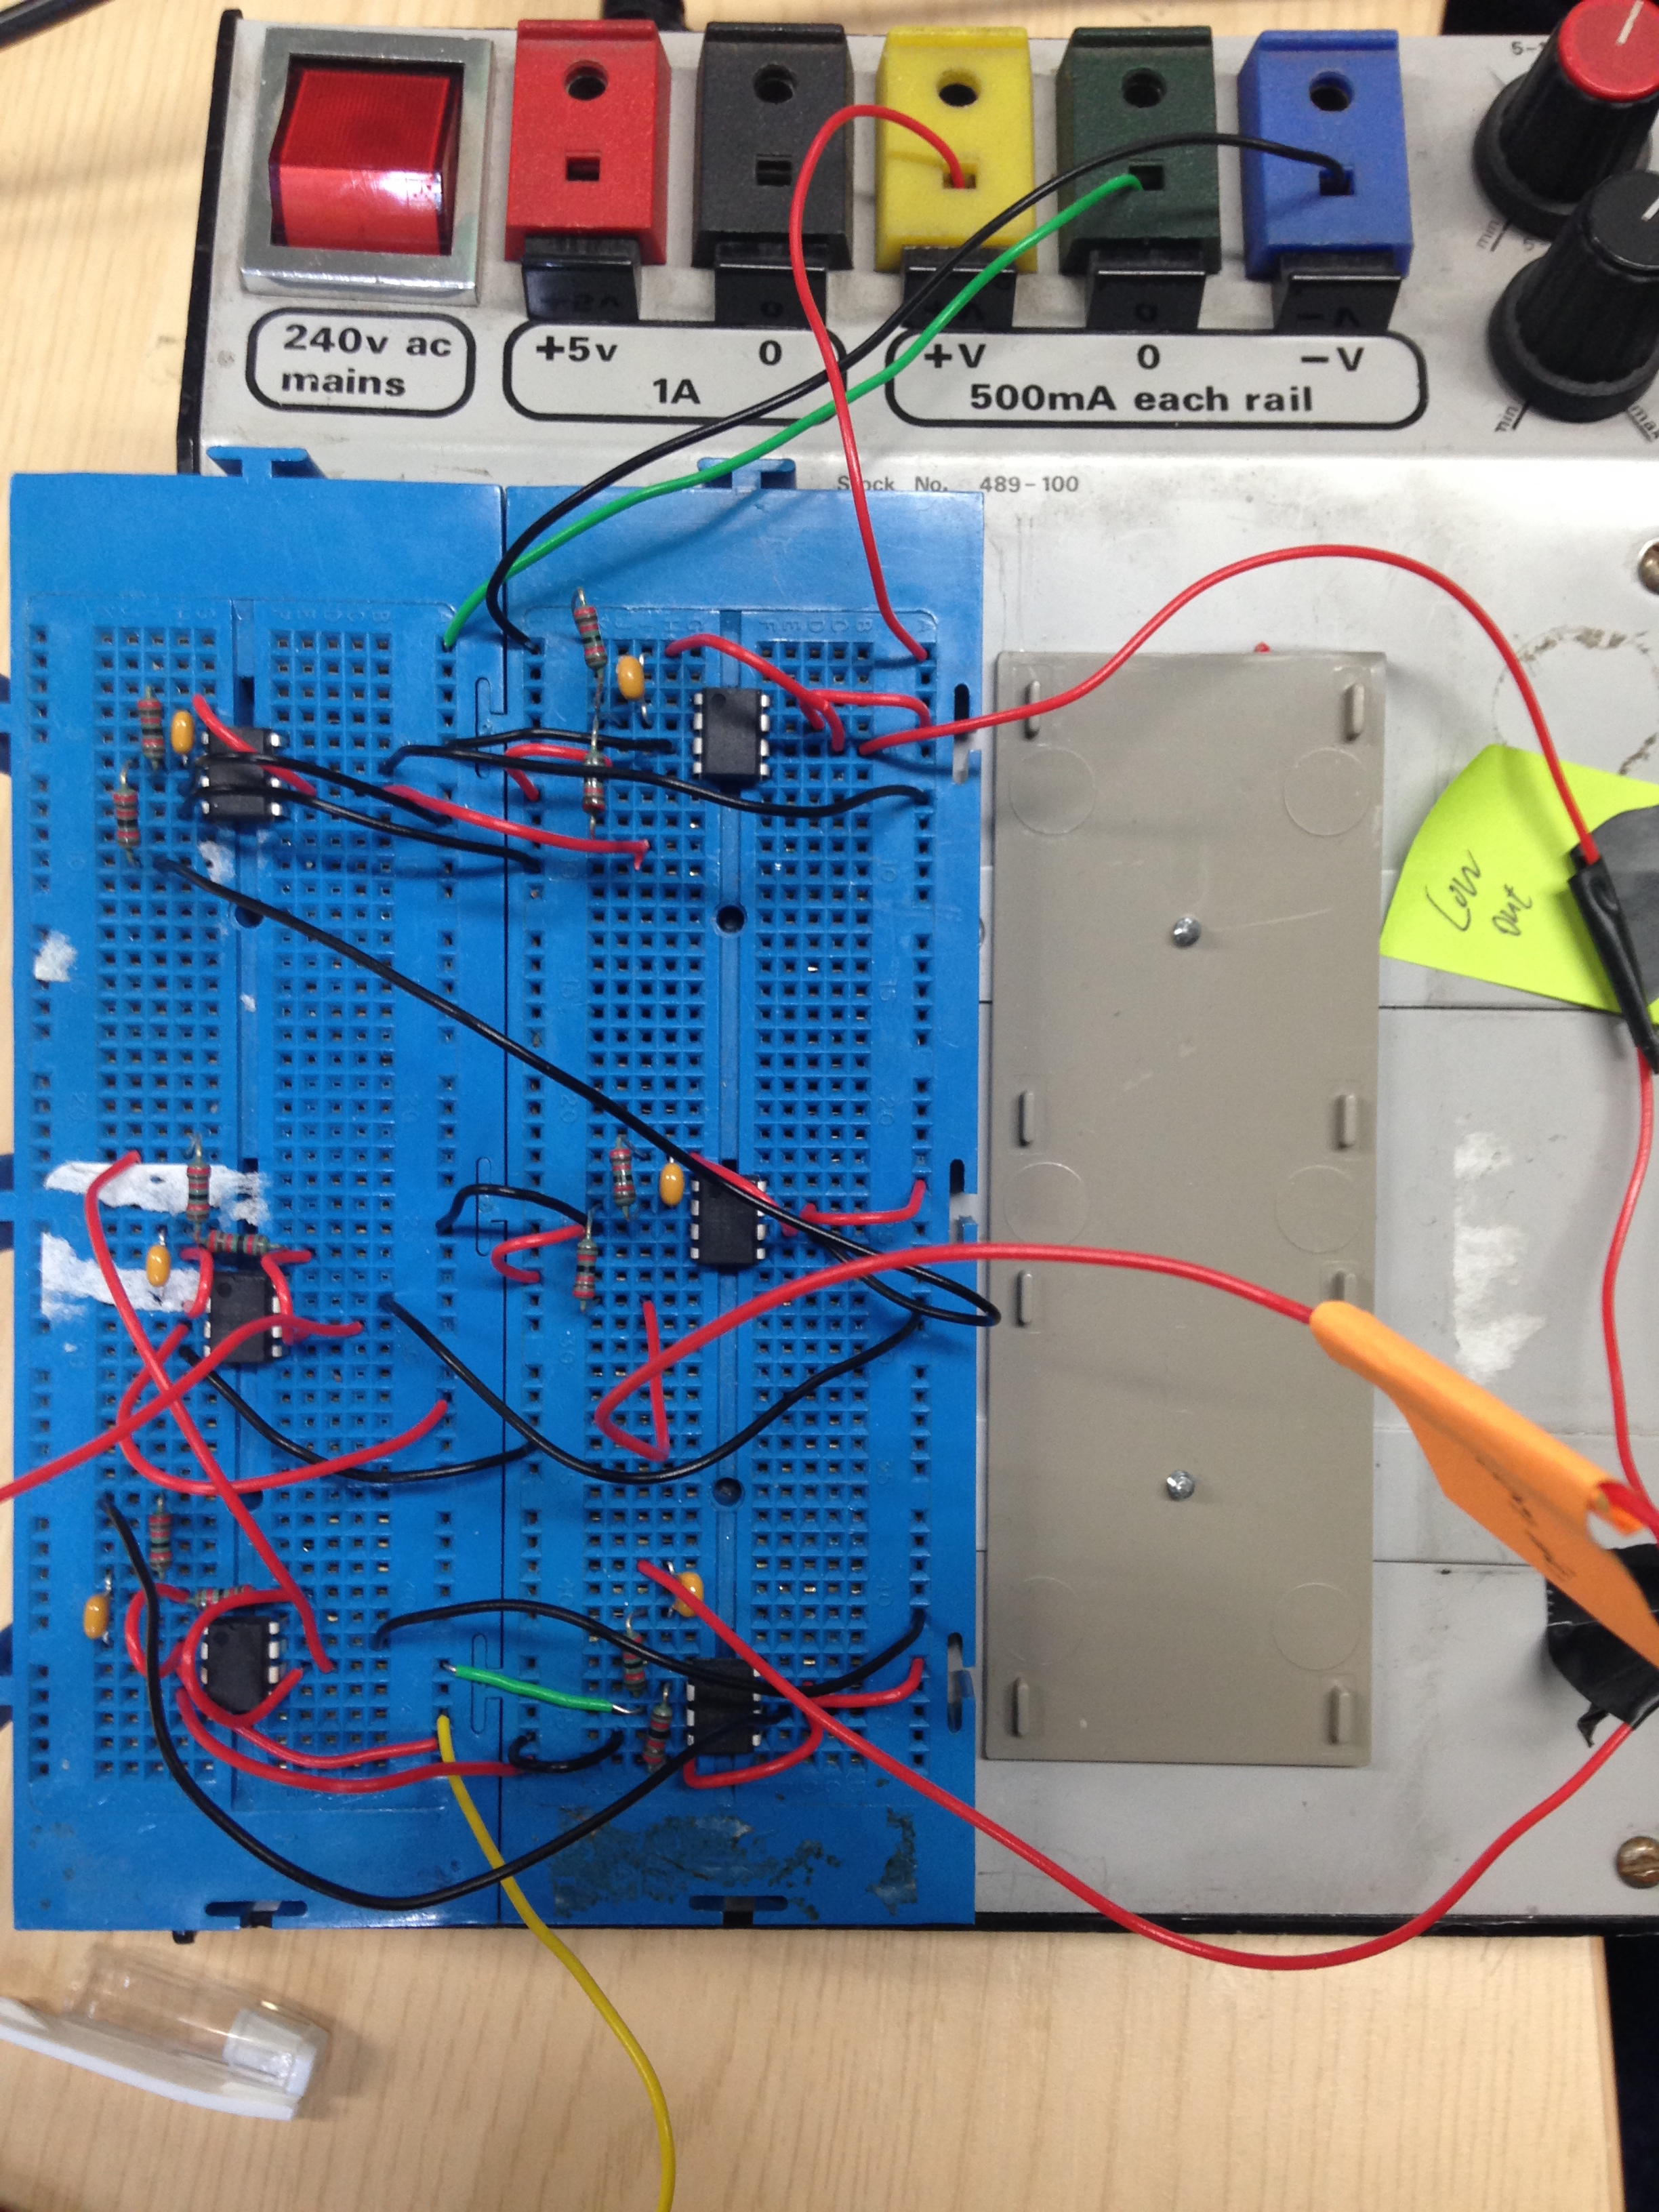
\includegraphics[scale = 0.1]{1383.JPG}
\captionof{figure}{This is the snapshot of the experiment board.}
}
\end{minipage}
\medskip
\end{center}

We adopted the value of resistor as $12k\Omega$ and the capacitor's value at 5.6uF. And the practical crossover frequency is at around 2368khz.
\subsection{The simulation result of the filter}
A python code is written to do the simulation of the experiment,
\begin{lstlisting}[language=Python]
# -*- coding: utf-8 -*-
"""
Created on Thu Mar 12 10:45:26 2015

@author: y1275963
"""

import numpy as np
import matplotlib.pylab as plt


# Low Pass Filter
def low_filter(f):
    w = 2*np.pi * f
    
    R = 12*10**3
    c = 5.6 * 10 **(-9)
    
    wh = 1.0/(R * c)
    h = -1/(1+1j*w/wh)
    
    print "Lowpass : The numerical cutoff frequency:", max(f[np.where(abs(h)>0.707)])
    return h

def high_filter(f):
    w = 2*np.pi * f
    
    R = 12*10**3
    c = 5.6 * 10 **(-9)
    
    wl = 1.0/(R * c)
    h = -1j*w*c*R/(1+1j*w/wl)
    
    print "Highpass : The numerical cutoff frequency:", min(f[np.where(abs(h)>0.707)])

    return h

    

if __name__ == "__main__":
    f = np.arange(0,10000,0.1)
    s_low = low_filter(f)
    m_low = s_low**3
    s_high = high_filter(f)
    m_high = s_high ** 3
    plt.plot(f,abs(s_low),label = "signal_high_pass")
    plt.plot(f,abs(s_high),label = "signal_low_pass")
    plt.plot(f,abs(m_low),label="3rd low")
    plt.plot(f,abs(m_high),label = "3rd high")
    plt.plot(f,abs(m_low + m_high),label = 'cross_over_filter')
   # plt.xscale('log')
    #plt.yscale('log')
    plt.legend(bbox_to_anchor=(0., 1.02, 1., .102), loc=3,
           ncol=2, mode="expand", borderaxespad=0.)
\end{lstlisting}
Below is the result:
\begin{center}
\begin{minipage}[t]{\linewidth}
%\label{fig:main}

{
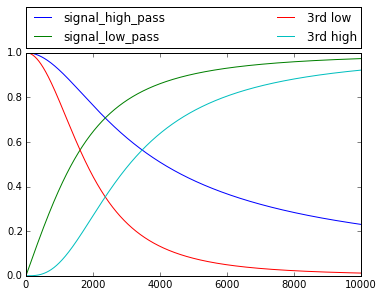
\includegraphics[scale = 1]{sim.png}
\captionof{figure}{This is the Simulation result.}
}
\end{minipage}
\medskip
\end{center}

 Below is the simulation result:
\begin{verbatim}
Lowpass : The numerical cutoff frequency: 2369.0
Highpass : The numerical cutoff frequency: 2367.7
\end{verbatim}
\subsection{The practical result of the filter}
We used signal generator and oscilloscope to test the filter. 
Below is the low pass filter's data:\\
\begin{center}
\begin{tabular}{|l|l|l|}
\hline
frequency&input voltage(mv)&output voltage(mv)\\\hline
100&560&560\\\hline
300&560&540\\\hline
500&560&520\\\hline
700&560&480\\\hline
900&560&460\\\hline
1100&560&420\\\hline
1300&540&360\\\hline
1500&540&340\\\hline
1700&540&320\\\hline
1900&540&280\\\hline
2100&540&240\\\hline
2300&540&200\\\hline
2500&540&180\\\hline
2700&540&160\\\hline
2900&540&140\\\hline
3100&540&130\\\hline
3300&540&120\\\hline
3500&540&110\\\hline
3700&540&100\\\hline
3900&540&90\\\hline
4100&540&80\\\hline
4500&540&70\\\hline
4900&540&60\\\hline
\end{tabular}
\end{center}

Below is the high pass filter's data:\\
\begin{center}
\begin{tabular}{|l|l|l|}
\hline
frequency&input voltage(mv)&output voltage(mv)\\\hline

100&560&24\\\hline
300&544&32\\\hline
500&552&40\\\hline
700&552&64\\\hline
900&544&80\\\hline
1100&552&112\\\hline
1500&544&176\\\hline
1700&544&200\\\hline
1900&544&232\\\hline
2100&544&256\\\hline
2300&544&272\\\hline
2500&544&300\\\hline
2700&544&320\\\hline
2900&544&340\\\hline
3100&540&360\\\hline
3300&540&380\\\hline
3500&540&390\\\hline
3700&540&400\\\hline
3900&540&420\\\hline
4400&540&440\\\hline
4900&540&460\\\hline
\end{tabular}

\end{center}

This is the plot:
\begin{center}
\begin{minipage}[t]{\linewidth}
%\label{fig:main}

{
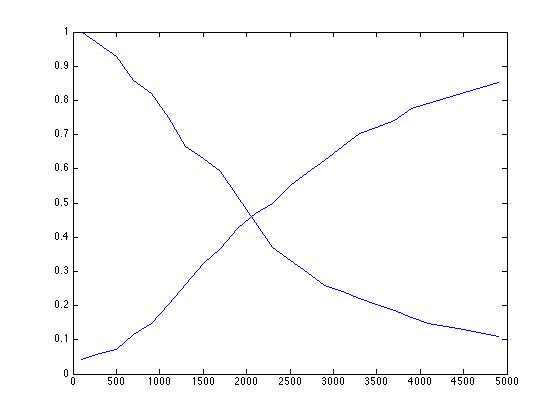
\includegraphics[scale = 0.7]{cross.jpg}
\captionof{figure}{This is the plotting of the filter's respose}
}
\end{minipage}
\medskip
\end{center}

As we can see from the graph, the filters cross at around 2.3khz, which is corrects, and we get the response's attenuation ratio at around 0.35 which is correct as well( It is a third order system). The graph is very similar to the simulation result.
\section{Comparison of the two speakers}

To put the filter in the test we connected the lower part of the filter to the woofer and higher part of the filter to the tweeter. And we use the CLIO to do the sinusoidal test. The speaker is enclosed in the case and the distance in between the speaker and microphone is in the medium range. 

\begin{center}
 \begin{minipage}[t]{\linewidth}
 %\label{fig:main}
 
 {
 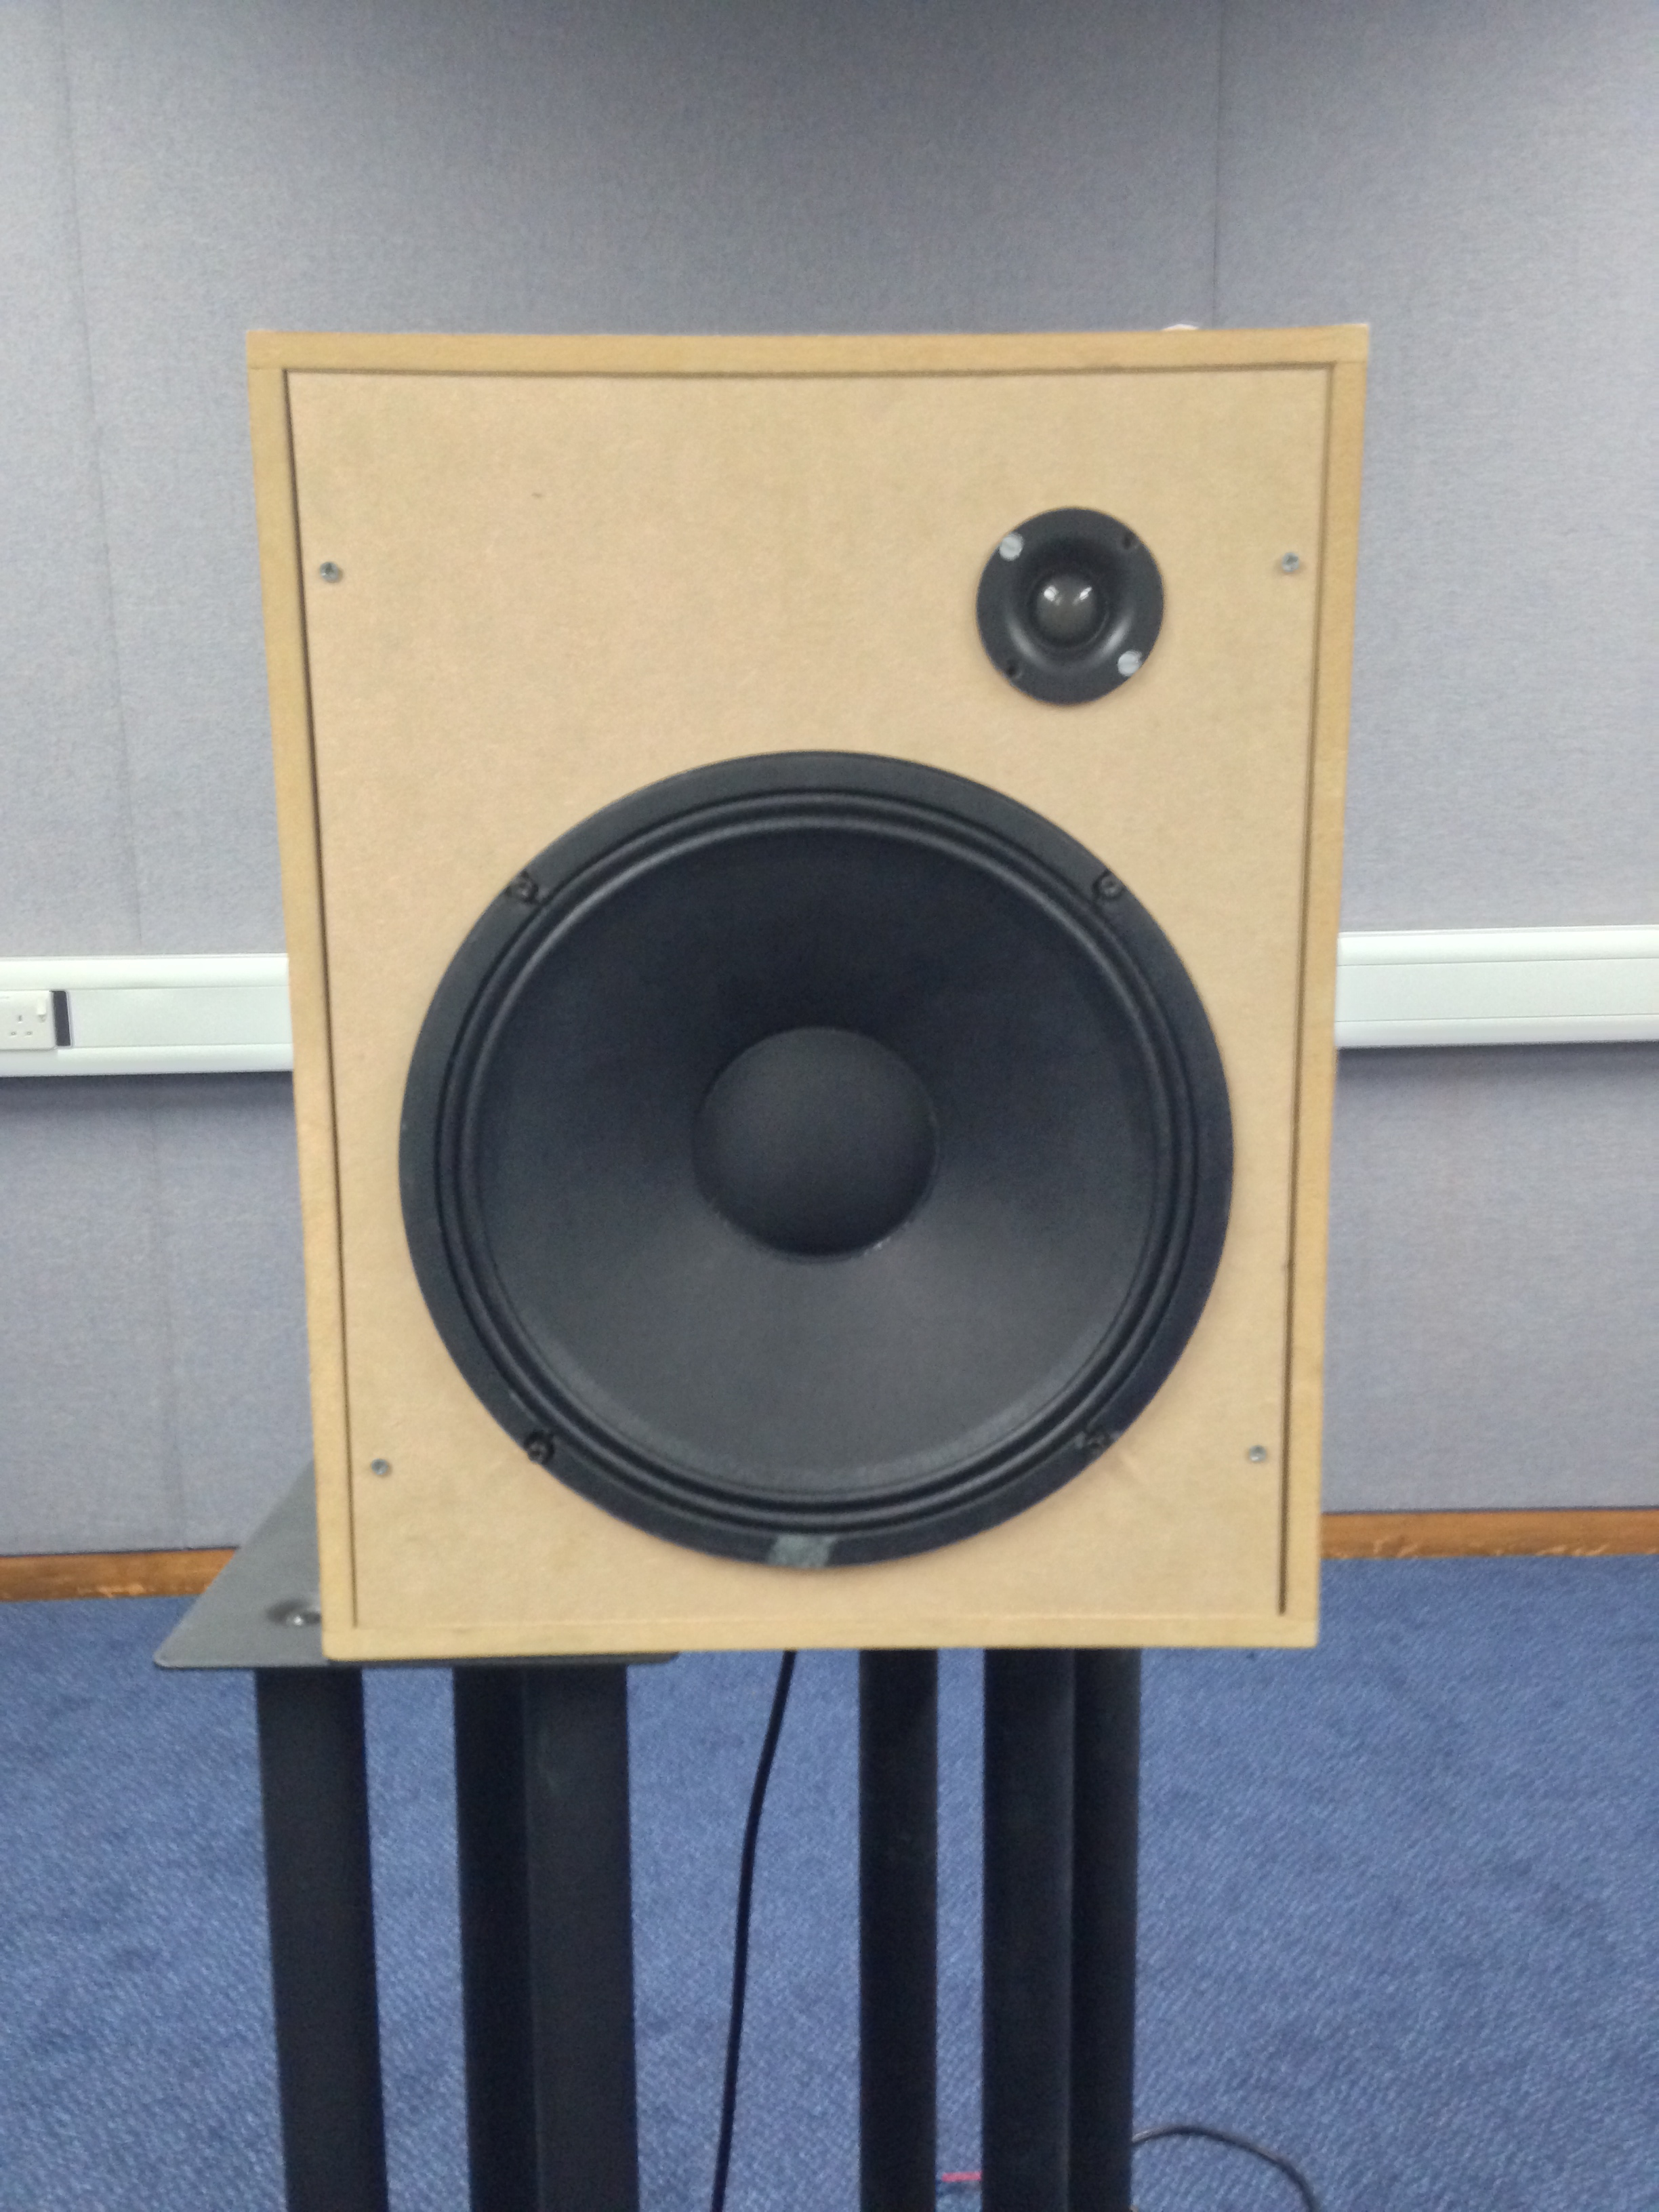
\includegraphics[scale = 0.1]{1385.JPG}
 \captionof{figure}{This is the experiment setup.}
 }
 \end{minipage}
 \medskip
 \end{center}


Below is the image of the speaker with active filter:
\begin{center}
\begin{minipage}[t]{\linewidth}
%\label{fig:main}

{
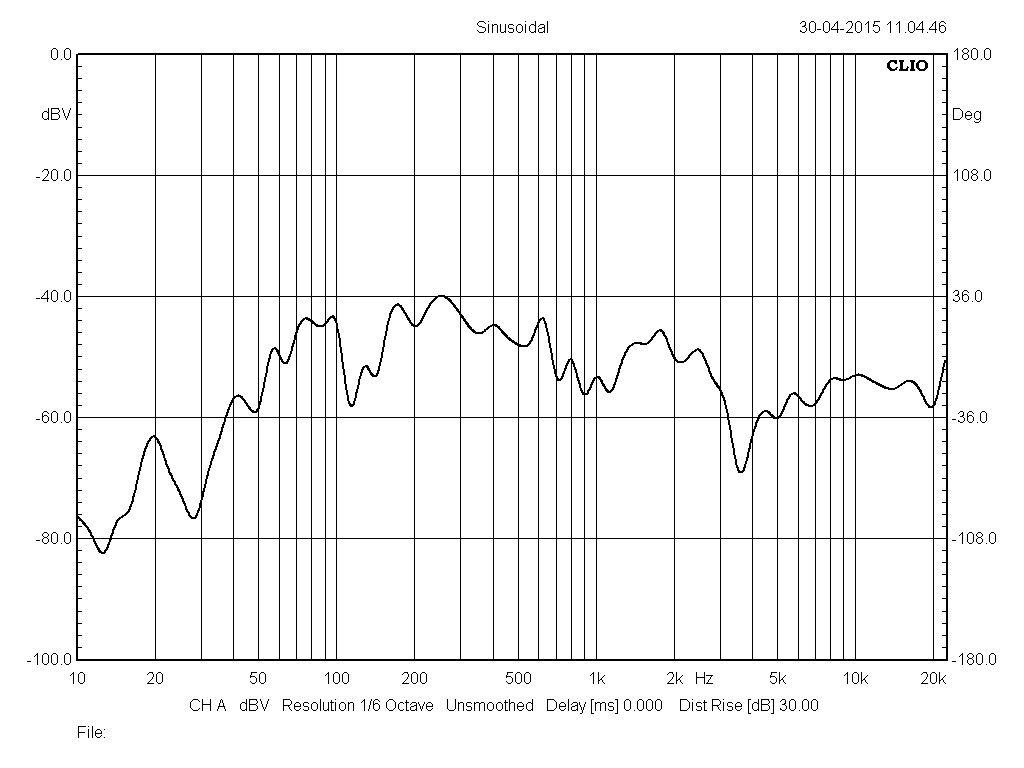
\includegraphics[scale = 0.3]{passive.png}
\captionof{figure}{This is the frequency response of the passive filter.}
}
\end{minipage}
\medskip
\end{center}
Below is the image of the speaker with passive filter:
\begin{center}
\begin{minipage}[t]{\linewidth}
%\label{fig:main}

{
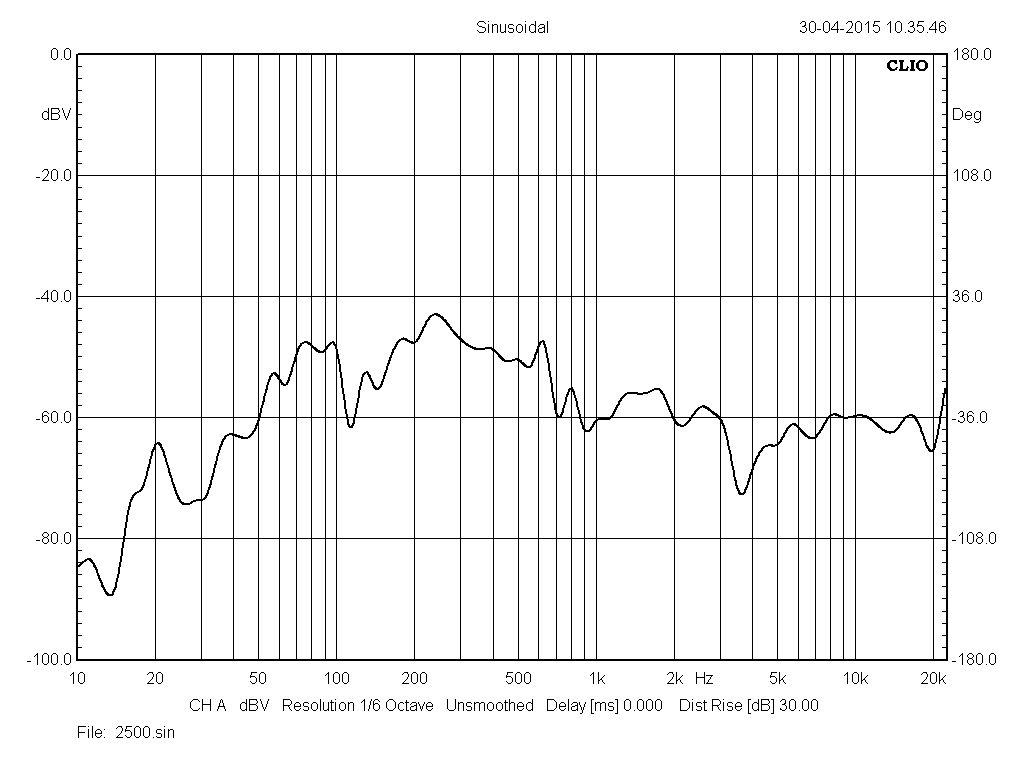
\includegraphics[scale = 0.3]{active.jpg}
\captionof{figure}{This is the frequency response of the active filter.}
}
\end{minipage}
\medskip
\end{center}

As we can see, those two almost have identical response figure and it is hard to distinguish them in between, and overall the passive filter has a lower variance and a slightly flatten response. But they are almost the same in terms of the frequency response's turning points.

Because we are afraid that the high frequency components in the testing signal will damage the tweeter we didn't do the experiment of the both speaker's response without filter.


\end{document}
